\subsection{Fundamentally Different Projects} \label{subsection:eval_diff_projects}

\subsubsection{Longer Training Rounds with more Learners}

Figure \ref{fig:eval_2_cpu_mem} shows the CPU and memory utilization of experiment (2).
Because this project configuration uses more learners and training rounds, it is logical that the FL training stage will last longer.
Note that this larger example is still relatively small compared to ML/FL training periods that take multiple hours or days to complete.
The CPU utilization during training is less spread than for (1) and concentrates in the high 90-100\% range.
Memory shows a similar shift from the low 60s to the low 70s.
The disk space and net-IO stay similar to (1).
The resulting accuracies are now all in the mid-80s instead of below 80\%.
Extended training periods lead to better results in this case.

\begin{figure}[t]
    \begin{adjustwidth}{-0.2\paperwidth}{-0.2\paperwidth}
        \centering
        % 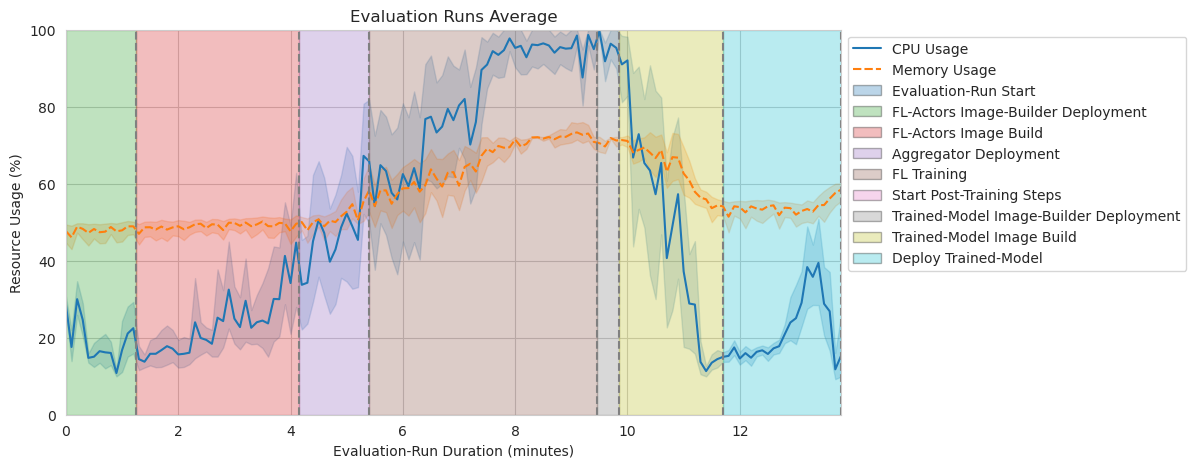
\includegraphics[width=0.85\paperwidth]{eval_2_simple_large_cpu_and_mem.png}
        \includegraphics[width=0.90\paperwidth]{evaluations/experiment_2/cpu_mem.pdf}
        \caption{Experiment 2: CPU \& Memory}
        \label{fig:eval_2_cpu_mem}
    \end{adjustwidth}
\end{figure}

\subsubsection{Different ML Repository, Framework, and Dataset}
Figure \ref{fig:eval_5_cpu_mem} shows the CPU and memory utilization of experiment (5).
The first noticeable difference to (1) is the almost threefold project duration, mainly due to build times.
Pytorch is a more heavy-weight ML library than Scikit-learn.
Thus, configuring its larger dependencies takes longer.
(5)'s CPU behavior is similar to (1).
The FL training in (5) requires less memory (mid 50s) than in (1) (low 60s).

Figure \ref{fig:eval_5_disk_space} shows the remarkable influence of the chosen ML framework and its dependencies for FLOps.
Compared to the relatively lightweight Sklearn base-case example with a total used disk space increase of 14 GB, this simple Pytorch example takes up approximately 35 GB in the end.
During build times when dependencies are pulled, the peak extra disk space utilization reaches 60 GB.
These heavy dependencies are also visible in the network IO in Figure \ref{fig:eval_5_net_io}.
The garbage collection is strongly present and visible in this case.
The tiny number of learners and training rounds lead to a small accuracy of 40\% of the final models.

\begin{figure}[p]
    \begin{adjustwidth}{-0.2\paperwidth}{-0.2\paperwidth}
        \centering
        % 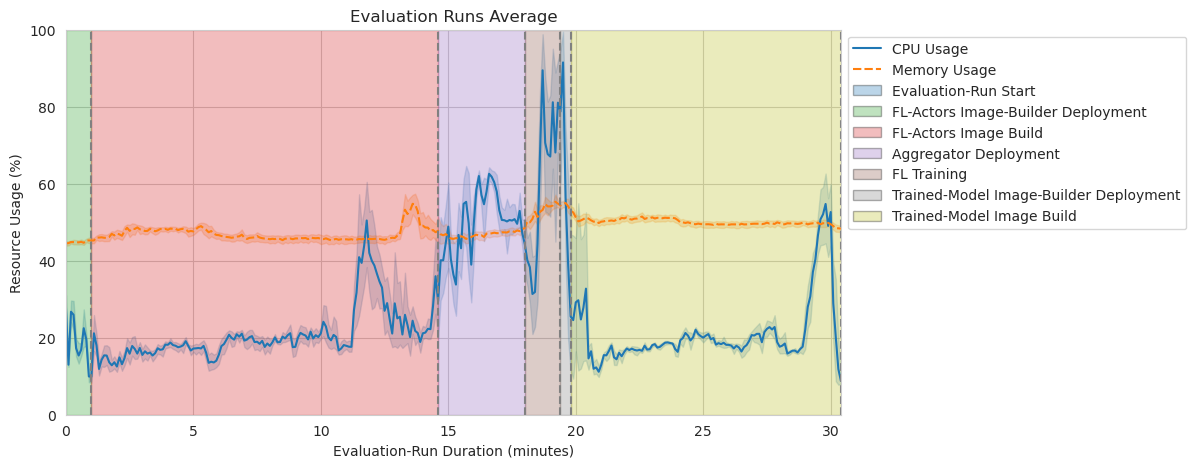
\includegraphics[width=0.80\paperwidth]{eval_5_simple_pytorch_cpu_and_mem.png}
        \includegraphics[width=0.85\paperwidth]{evaluations/experiment_5/cpu_mem.pdf}
        \caption{Experiment 5: CPU \& Memory}
        \label{fig:eval_5_cpu_mem}
    \end{adjustwidth}

    \begin{adjustwidth}{-0.2\paperwidth}{-0.2\paperwidth}
        \centering
        % 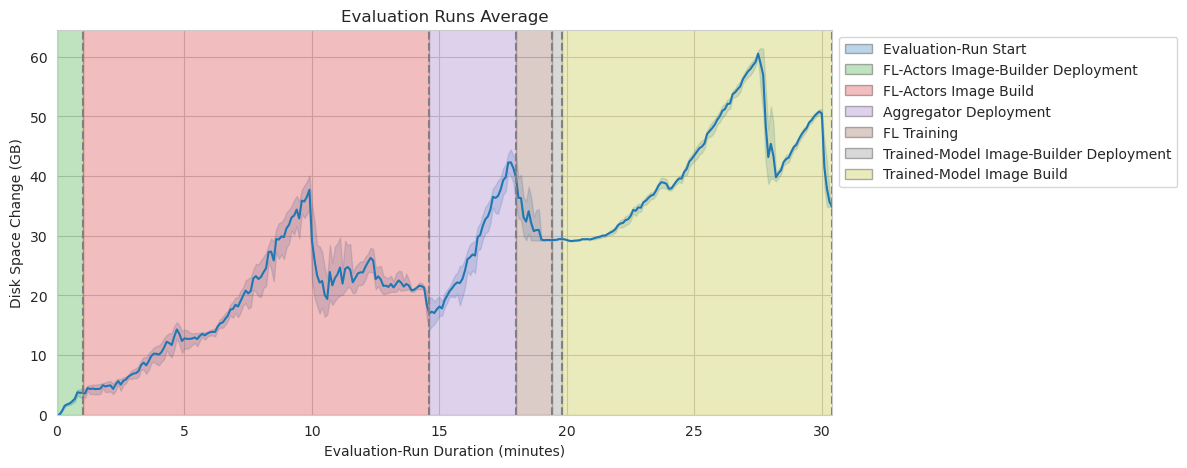
\includegraphics[width=0.80\paperwidth]{eval_5_simple_pytorch_disk_space.png}
        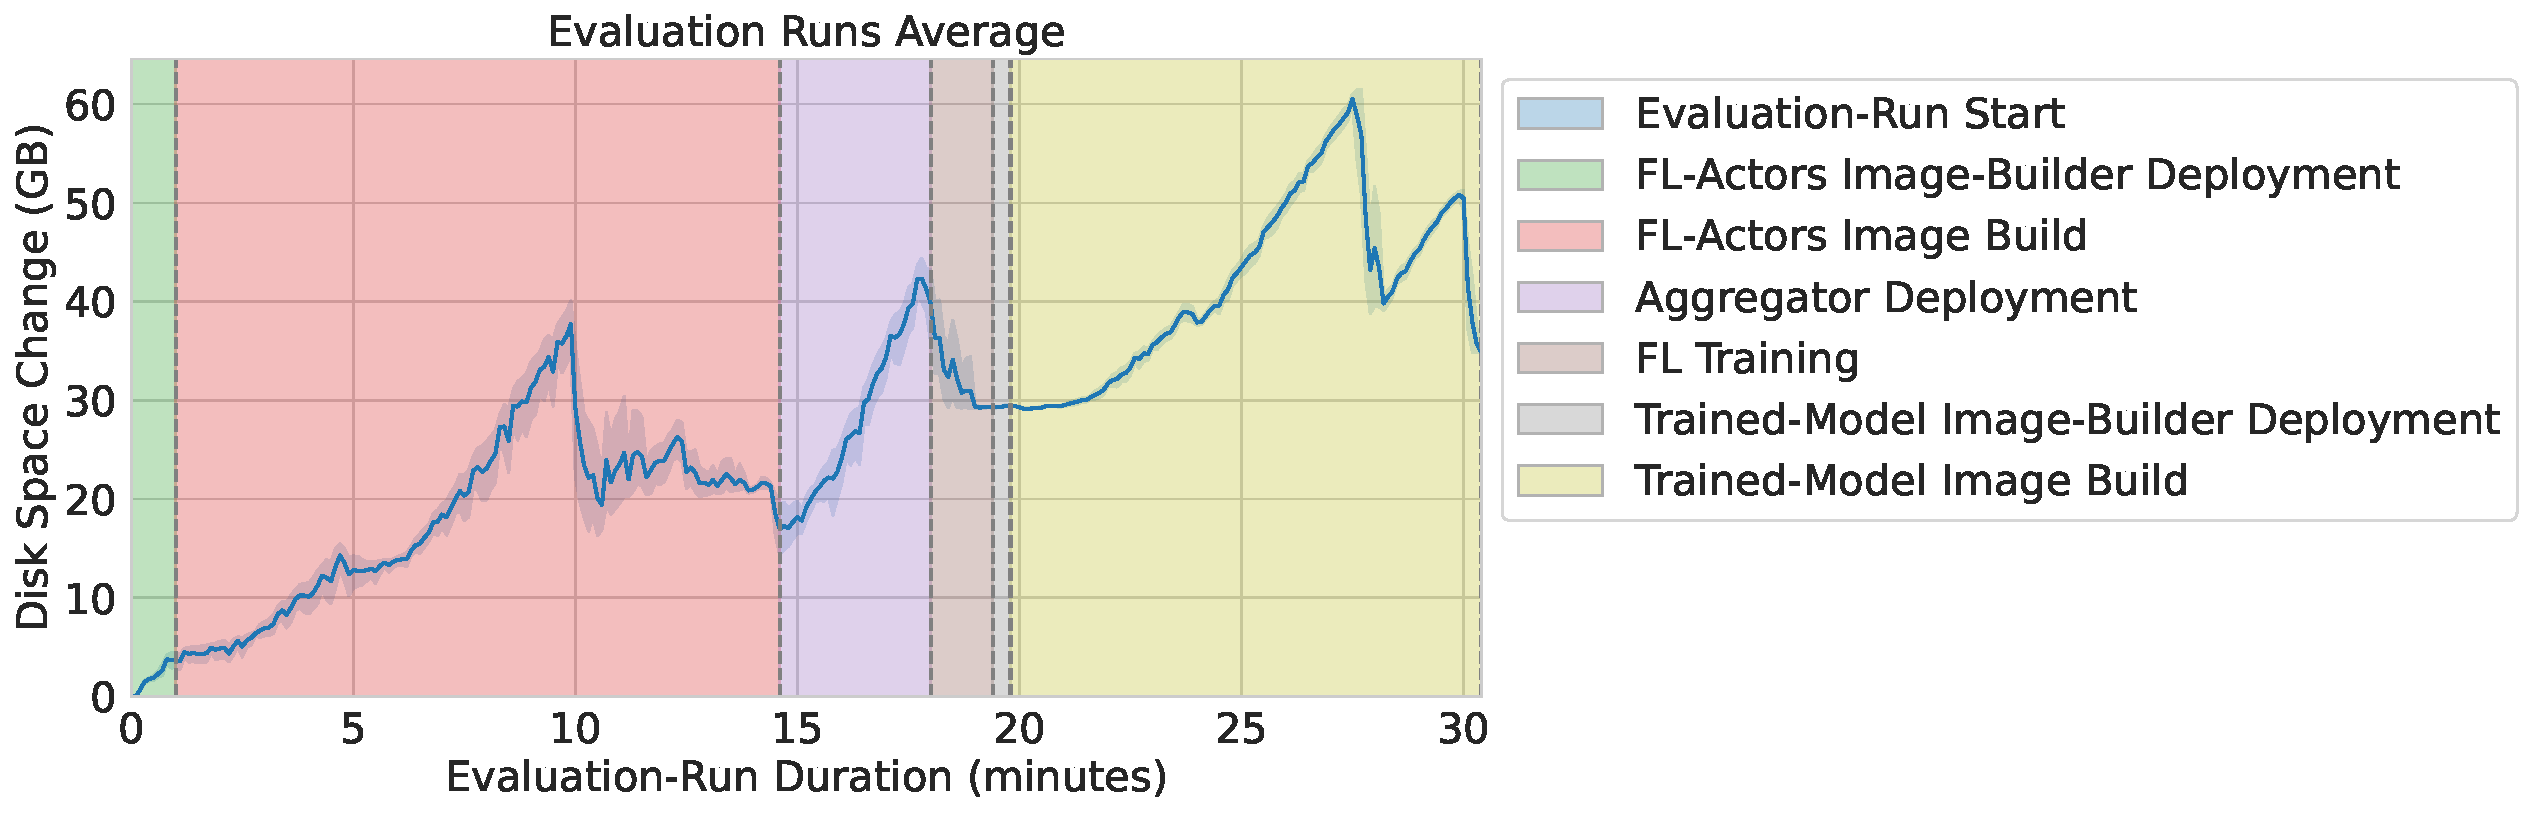
\includegraphics[width=0.85\paperwidth]{evaluations/experiment_5/disk_linear.pdf}
        \caption{Experiment 5: Disk Space}
        \label{fig:eval_5_disk_space}
    \end{adjustwidth}

    \begin{adjustwidth}{-0.2\paperwidth}{-0.2\paperwidth}
        \centering
        % 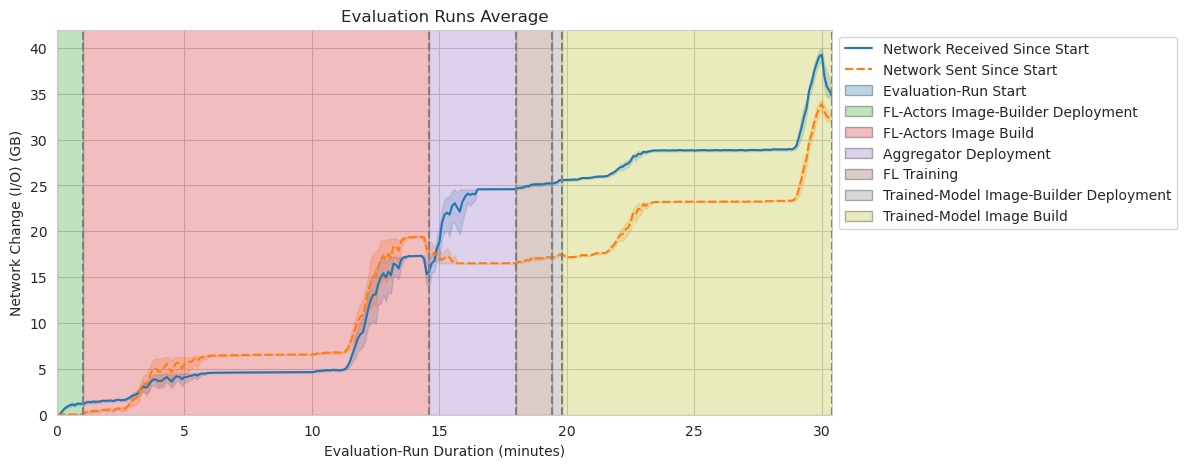
\includegraphics[width=0.80\paperwidth]{eval_5_simple_pytorch_net_io.png}
        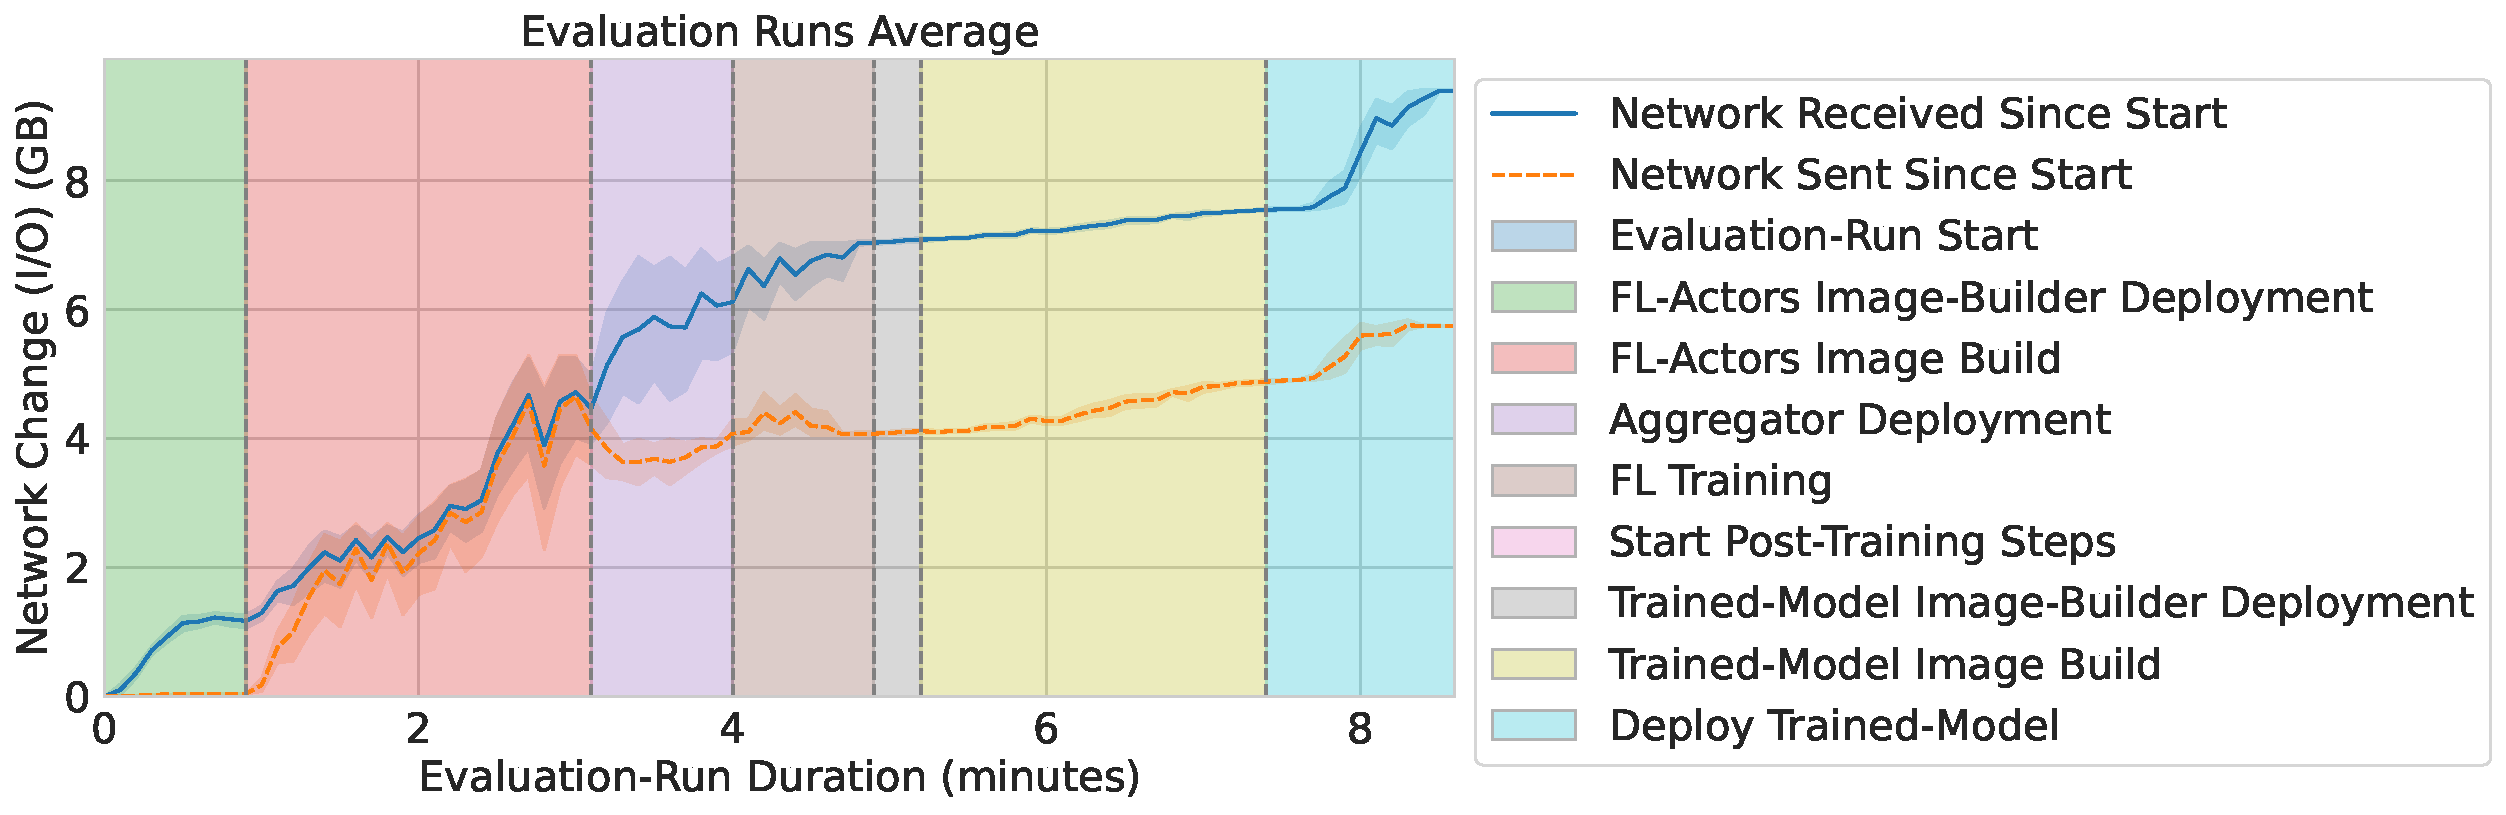
\includegraphics[width=0.85\paperwidth]{evaluations/experiment_5/net_io.pdf}
        \caption{Experiment 5: Network IO}
        \label{fig:eval_5_net_io}
    \end{adjustwidth}
\end{figure}

These experiments prove that FLOps can handle different FL training configurations using various ML frameworks, repositories, and datasets.
They also unveil that using popular classic ML libraries might be unrealistic for resource-constrained edge devices.
Thus, libraries that are dedicated to restricted devices should be analyzed and tried out as future work.

% \pagebreak
